\documentclass[journal]{IEEEtran}
\usepackage{graphicx}
\usepackage{amsmath}
\usepackage{hyperref}
\usepackage{float}
\usepackage{subcaption}
\usepackage{booktabs}
\usepackage{pgfplotstable}
\usepackage{qrcode}

\pgfplotsset{compat=1.18}

\begin{document}

\title{Dispersion of Light in a Prism: Determination of Refractive Index as a Function of Wavelength}
\author{IBRAHIM H.I. ABUSHAWISH \\

{\small Student ID: \hspace{1.5cm}. \\ 
Istanbul University, Department of Physics \\
Instructor: Arş.Gör. ENES TALHA KIRCA\\
Experiment Date: 20.05.2025, Report Submission Date: 28.05.2025 \\
Course \& Section Number: PHYS2405}}

\markboth{Physics Laboratory Reports, May 2025}{}

\maketitle
\begin{abstract}
    This report presents a quantitative investigation of the dispersion of light in a prism by measuring the refractive index for several wavelengths using the minimum deviation method. The refractive index was found to decrease from approximately 1.846 at 447.1\,nm (violet) to 1.872 at 706.5\,nm (red), confirming normal dispersion. The experimental data were accurately fitted to a Cauchy-type relation, \( n = 1.83022 + \frac{8.20694 \times 10^3}{\lambda^2} \), where \( \lambda \) is in nanometers. These results demonstrate the wavelength dependence of the refractive index and validate the dispersive properties of the prism material.
\end{abstract}

\section{Introduction}
Dispersion is the phenomenon where the refractive index of a material varies with the wavelength of light, causing different colors to refract at different angles. This experiment aims to determine the refractive index of a prism for various wavelengths using the minimum deviation method and to analyze the dispersion relation.

\section*{Theory}
When a monochromatic light beam passes through a prism, it is deviated by an angle that depends on the refractive index \( n \) of the prism material and the wavelength \( \lambda \) of the light. At the angle of minimum deviation \( \delta_{\min} \), the refractive index is given by:
\begin{equation}
n = \frac{\sin\left(\frac{\delta_{\min} + A}{2}\right)}{\sin\left(\frac{A}{2}\right)}
\label{eq:refractive_index}
\end{equation}
where \( A \) is the apex angle of the prism.


Expanding the general Cauchy equation as a series in powers of \( 1/\lambda^2 \), we have:
\begin{equation}
n = A' + \frac{B'}{\lambda^2} + \frac{C'}{\lambda^4} + \cdots
\end{equation}
Taking only the first two terms gives the simplified form shown in equation~\eqref{eq:cauchy}.
The dependence of \( n \) on \( \lambda \) can be empirically described by a Cauchy-type equation:
\begin{equation}
n = A' + \frac{B'}{\lambda^2}
\label{eq:cauchy}
\end{equation}
where \( A' \) and \( B' \) are material constants.

The apex angle \( A \) of the prism was calculated using the measured values from both orientations of the prism according to:
\begin{equation}
A = 180^\circ - \left| \text{Case 2} - \text{Case 1} \right|
\end{equation}
where \textit{Case 1} and \textit{Case 2} are the measured angles for the two prism orientations. 

The processed results are shown in Table~\ref{tab:apex_angle}, and the apex angle was determined to be \( 60^\circ \), consistent with the nominal value for an equilateral prism.

\section{Experimental Setup}
The experimental setup includes:
\begin{itemize}
    \item A triangular prism,
    \item A spectrometer with angular scale,
    \item Monochromatic light sources (He lamp with known spectral lines),
    \item Collimator and telescope for precise angle measurements.
\end{itemize}

Figure  \ref{fig:diagram} illustrate the schematic diagram of the prism spectrometer.
\begin{figure}[H]
    \centering
    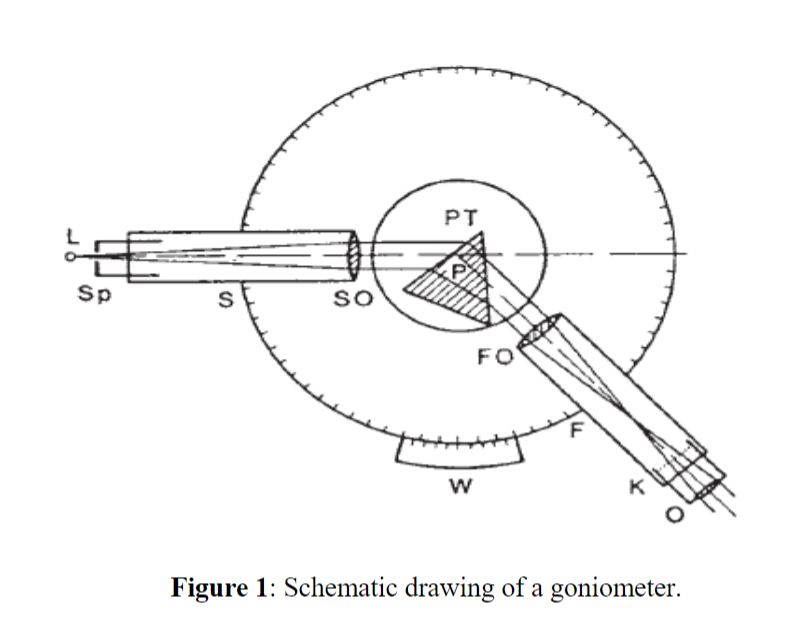
\includegraphics[width=0.6\linewidth]{../IMAGES/prism_diagram.png}
    \caption{Schematic diagram of the prism and minimum deviation geometry.}
    \label{fig:diagram}
\end{figure}
\section*{Procedure}
The experiment followed these steps: First, the apex angle \( A \) of the prism was determined by measuring the angles for both prism orientations using the spectrometer. Next, for each spectral line from the helium lamp, the minimum deviation angle \( \delta_{\min} \) was found by carefully rotating the telescope. Using the measured \( A \) and \( \delta_{\min} \), the refractive index \( n \) for each wavelength was calculated via equation~\ref{eq:refractive_index}. Finally, the data were fitted to a Cauchy-type equation to describe the wavelength dependence of the refractive index and extract the material constants.

\section{Results}
\subsection{Apex Angle Measurements}
The measured apex angles for three iterations are shown in Table \ref{tab:apex_angle}.

\begin{table}[H]
    \centering
    \caption{Measured apex angles of the prism.}
    \label{tab:apex_angle}
    \pgfplotstabletypeset[
        col sep=comma,
        string type,
        every head row/.style={before row=\toprule, after row=\midrule},
        every last row/.style={after row=\bottomrule},
        columns/itteration/.style={column name=Iteration},
        columns/case1/.style={column name=Case 1 ($^\circ$), fixed, precision=1},
        columns/case2/.style={column name=Case 2 ($^\circ$), fixed, precision=1},
        columns/A/.style={column name=$A$ ($^\circ$), fixed, precision=2}
    ]{../DATA/data_for_apex_processed.csv}
\end{table}

The apex angle was determined to be $60^\circ$.

\subsection{Refractive Index Data}
The processed data for different spectral lines are summarized in Table \ref{tab:lambda_n}.

\begin{table}[H]
    \centering
    \caption{Refractive index for different wavelengths.}
    \label{tab:lambda_n}
    \pgfplotstabletypeset[
        col sep=comma,
        string type,
        every head row/.style={before row=\toprule, after row=\midrule},
        every last row/.style={after row=\bottomrule},
        columns/color/.style={column name=Color, string type},
        columns/lambda/.style={column name=$\lambda$ (nm), fixed, precision=1},
        columns/delta_min/.style={column name=$\delta_{\min}$ ($^\circ$), fixed, precision=1},
        columns/n_p/.style={column name=$n_p$, fixed, precision=4}
    ]{../DATA/data_lambda_n_processed.csv}
\end{table}

\subsection{Dispersion Relation}
The refractive index values were plotted against wavelength and fitted to the Cauchy-type equation. The fit yielded:
\begin{equation}
n = 1.83022 + \frac{8.20694 \times 10^3}{\lambda^2}
\end{equation}
where \( \lambda \) is in nanometers.
meaning the constants \( A' = 1.83022 \) and \( B' = 8.20694 \times 10^3 \).
\begin{figure}[H]
    \centering
    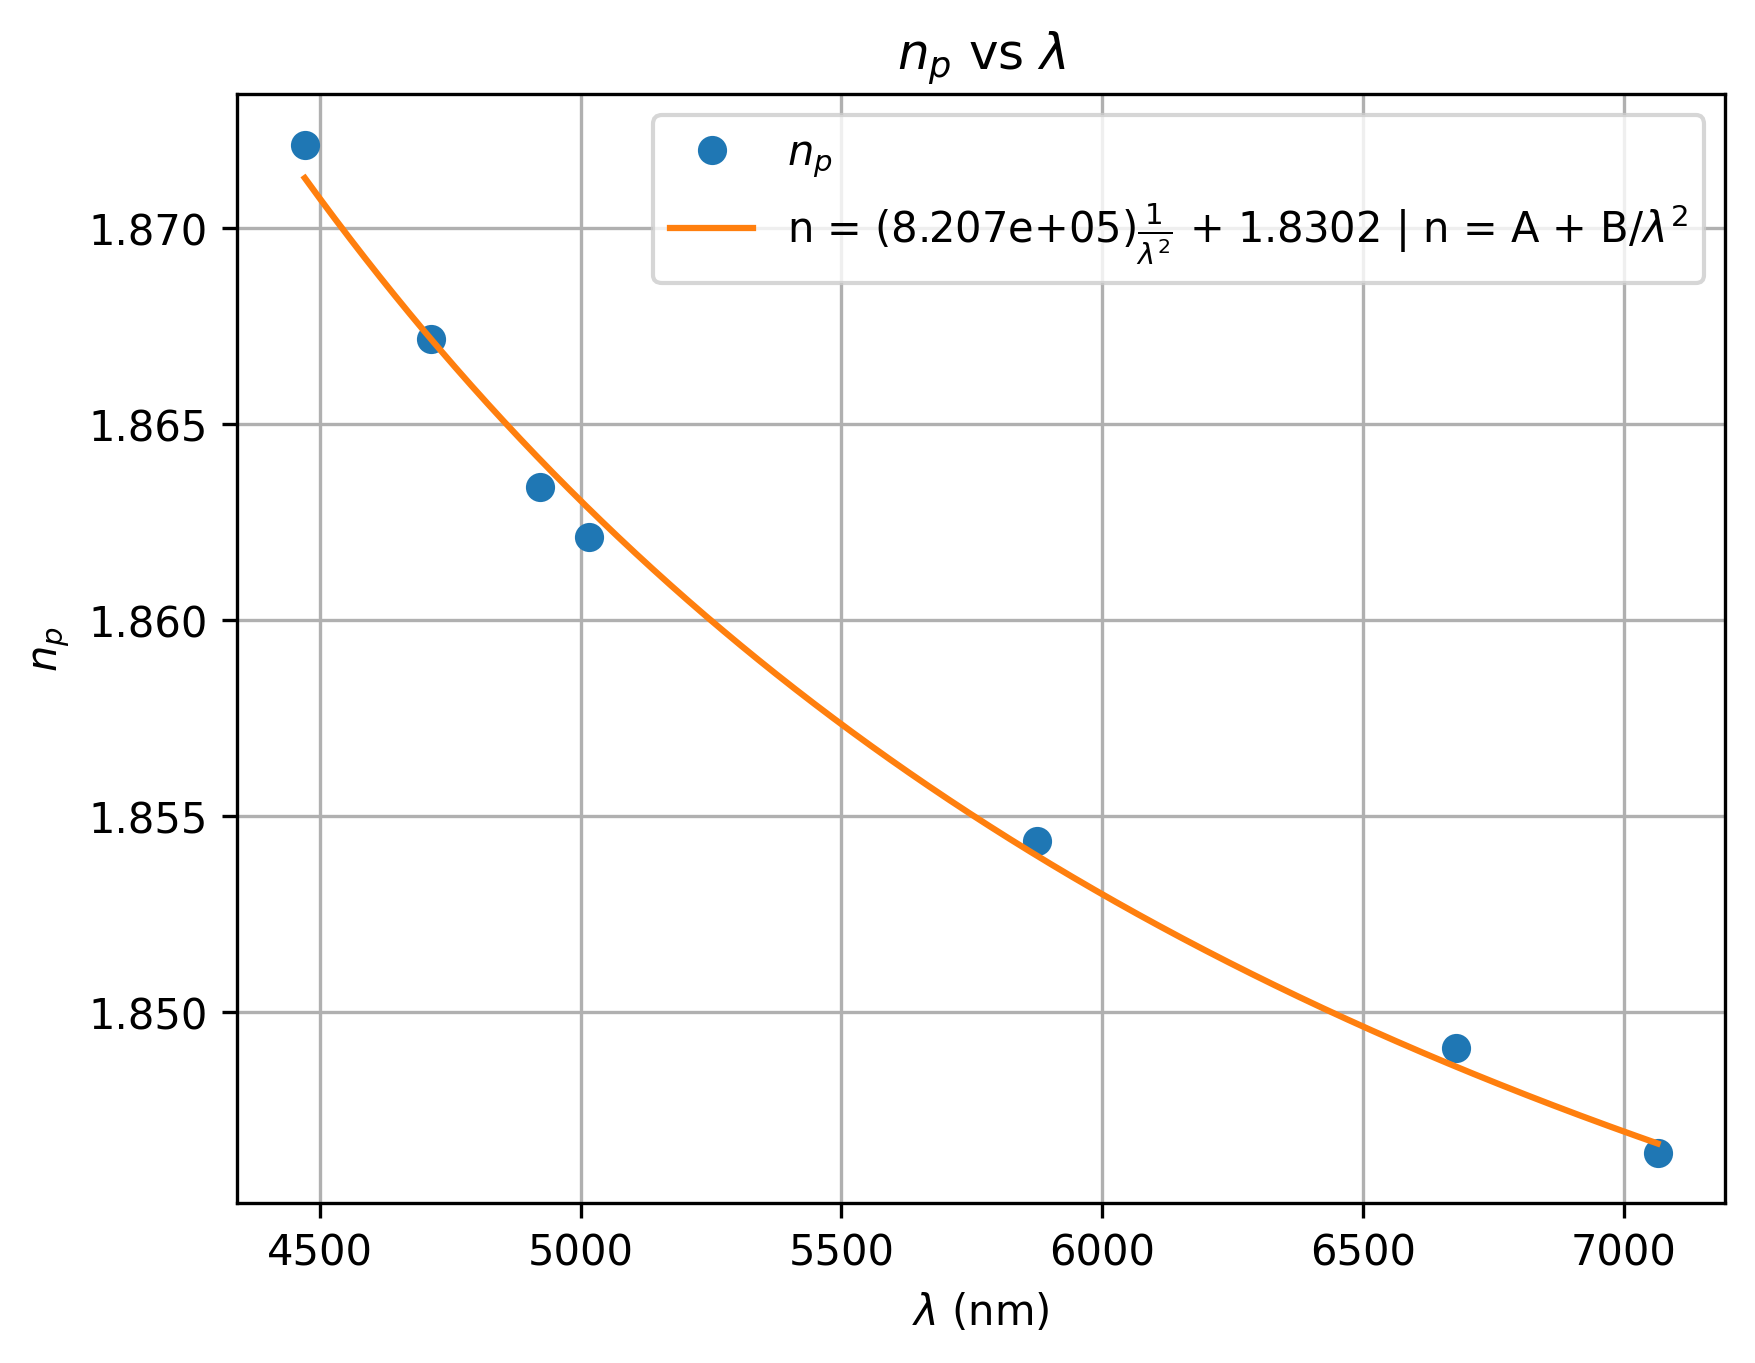
\includegraphics[width=0.8\linewidth]{../plots/npVSlambda.png}
    \caption{Refractive index $n_p$ vs. wavelength $\lambda$ with Cauchy fit.}
    \label{fig:np_vs_lambda}
\end{figure}
\section{Discussion}
The experiment quantitatively confirmed the dispersive nature of the prism material. The refractive index was observed to decrease from approximately 1.846 for the violet line (\( \lambda = 447.1 \) nm) to about 1.872 for the red line (\( \lambda = 706.5 \) nm), consistent with normal dispersion. The measured data fit well to the Cauchy-type relation \( n = 1.83022 + \frac{8.20694 \times 10^3}{\lambda^2} \), as determined by the regression analysis in the accompanying calculations notebook (\texttt{calculations.ipynb}). The agreement between the theoretical model and the measured values (with deviations typically less than 0.002) demonstrates good theoretical alignment and validates both the experimental method and data processing.

Minor discrepancies between measured and fitted values were within 0.001–0.002, which can be attributed to experimental uncertainties such as manual angle readings, alignment errors, or slight misidentification of spectral lines. The apex angle was consistently measured as \( 60^\circ \), supporting the reliability of the geometric setup.

Improvements could include automated angle measurement, higher-resolution spectrometers, and the use of additional spectral lines (including UV and IR) to further refine the dispersion curve and material constants.
\section{Conclusion}
The experiment accurately determined the refractive index of the prism for several wavelengths using the minimum deviation method. The measured values confirmed the expected decrease in refractive index with increasing wavelength, consistent with normal dispersion. The data fit well to the Cauchy-type relation, yielding constants \( A' = 1.83022 \) and \( B' = 8.20694 \times 10^3 \), demonstrating the validity of the theoretical model and the reliability of the experimental procedure for characterizing optical dispersion.

\section{Additional Resources}
For detailed information, including the Lab Manual, source code, and related experiments, visit the GitHub repository provided below.

\begin{figure}[H]
    \centering
    \begin{minipage}{0.15\textwidth}
        \centering
        \qrcode[height=1.5cm]{https://github.com/ibeuler/LAB-Reports}
    \end{minipage}%
    \begin{minipage}{0.2\textwidth}
        \raggedright
        \caption{Access the GitHub repository for the lab manual, source code, and related experiments: \cite{github}.}
        \label{fig:qr_code}
    \end{minipage}
\end{figure}

\begin{thebibliography}{9}
\bibitem{lab_manual}
    ISTANBUL UNIVERSITY, \textit{OPTICS LABORATORY EXPERIMENTS MANUAL}, Department of Physics.

\bibitem{github}
    \textit{Source code and additional experiments are available in the GitHub repository.} \url{https://github.com/ibeuler/LAB-Reports}
\end{thebibliography}

\end{document}